% !TEX root = ../main.tex

\section{Багатовимірний нормальний розподіл}
\subsection{Виведення характеристичної функції та щільності}

Розглянемо випадковий вектор $\vec{\xi} = (\xi_1, \xi_2, ..., \xi_n)^T$, $\xi_k \sim \mathrm{N}(a_k^o, \sigma_k)$ для $k=1,...,n$, координати незалежні у сукупності.
За властивостями характеристичної функції та щільності $\chi_{\vec{\xi}}(\vec{t}) = \prod\limits_{k=1}^n \chi_{\xi_k}(t_k)$,
$f_{\vec{\xi}}(\vec{x}) = \prod\limits_{k=1}^n f_{\xi_k}(x_k)$.

\begin{gather*}
    \chi_{\vec{\xi}}(\vec{t}) = \prod\limits_{k=1}^n e^{i a_k^o t_k - \frac{\sigma_k^2 t_k^2}{2}} = \exp\left\{i(\vec{a^o}, \vec{t}) - \frac{1}{2}\sum\limits_{k=1}^n \sigma_k^2 t_k^2\right\}
    \\
    f_{\vec{\xi}}(\vec{x}) = \prod\limits_{k=1}^n \frac{1}{\sqrt{2\pi}\sigma_k} e^{-\frac{(x_k-a_k^o)^2}{2\sigma_k^2}} = \frac{1}{(2\pi)^{n/2}\prod_{k=1}^n \sigma_k} \exp \left\{ -\frac{1}{2} \sum_{k=1}^n \frac{(x_k-a_k^o)^2}{\sigma_k^2}\right\}
\end{gather*}

Введемо матрицю $D = \begin{pmatrix}
    \sigma_1^2 & 0 & \cdots & 0 \\
    0 & \sigma_2^2 & \cdots & 0 \\
    \vdots & \vdots & \ddots & \vdots \\
    0 & 0 & \cdots & \sigma_n^2
\end{pmatrix}$, $D^{-1} = \begin{pmatrix}
    1/\sigma_1^2 & 0 & \cdots & 0 \\
    0 & 1/\sigma_2^2 & \cdots & 0 \\
    \vdots & \vdots & \ddots & \vdots \\
    0 & 0 & \cdots & 1/\sigma_n^2
\end{pmatrix}$.

\noindent Тоді отримаємо
\begin{gather}
    \chi_{\vec{\xi}}(\vec{t}) = \exp\left\{i(\vec{a^o}, \vec{t}) - \frac{1}{2}(D\vec{t}, \vec{t})\right\}
    \\
    f_{\vec{\xi}}(\vec{x}) = \frac{1}{(2\pi)^{n/2} \sqrt{{\det{D}}}} \exp \left\{ -\frac{1}{2} \left( D^{-1}(\vec{x} - \vec{a^o}), (\vec{x} - \vec{a^o})\right)\right\}
\end{gather}
Причому в такому випадку $D$ --- кореляційна матриця.

Тепер розглянемо вектор $\vec{\eta} = A\vec{\xi}$, де $A$ --- невироджена матриця. За властивістю 
$\chi_{\vec{\eta}}(\vec{t}) = \chi_{\vec{\xi}}(A^{*}\vec{t})$. Маємо
\begin{equation}
    \begin{gathered}
        \chi_{\vec{\eta}}(\vec{t}) = \exp\left\{i(\vec{a^o}, A^{*}\vec{t}) - \frac{1}{2}(DA^{*}\vec{t}, A^{*}\vec{t})\right\} =
    \exp\left\{i(A\vec{a^o}, \vec{t}) - \frac{1}{2}(ADA^{*}\vec{t}, \vec{t})\right\} = \\
    = \exp\left\{i(\vec{a}, \vec{t}) - \frac{1}{2}(K\vec{t}, \vec{t})\right\}
    \end{gathered}
\end{equation}
Доведемо, що $K = ADA^{*}$ --- симетрична й додатно визначена, тому її можна вважати кореляційною матрицею.
\begin{enumerate}
    \item $K^{*} = \left( ADA^{*}\right)^{*} = \left( A^{*}\right)^{*}DA^{*} = ADA^{*} = K$.
    \item $\forall \;\vec{u} \in \mathbb{R}^n$ $\left( K \vec{u}, \vec{u}\right) = \left( ADA^{*} \vec{u}, \vec{u}\right) =
    \left( DA^{*} \vec{u}, A^{*}\vec{u}\right) = \left[ A^{*}\vec{u} = \vec{v}\right] = \left( D\vec{v}, \vec{v}\right) > 0$ для $\vec{u}\neq \vec{0}$.
\end{enumerate}

Нехай в $n$-вимірному евклідовому просторі задано вектор $\vec{a}$ та симетричну додатно визначену матрицю $K$.
Існує ортогональне перетворення $U$, яке дає можливість записати $K=UDU^{*}$, причому на діагоналі $D$ стоять строго додатні
власні числа $K$. Тоді функцію вигляду $\exp\left\{i(\vec{a}, \vec{t}) - \frac{1}{2}(K\vec{t}, \vec{t})\right\}$ 
можна розглядати як характеристичну функцію випадкового вектора $\vec{\eta} = U \vec{\xi}$, де $\vec{\xi}$ ---
вектор, координати якого незалежні у сукупності та мають нормальний розподіл.

\begin{definition}
    $n$\emph{-вимірним гауссівським вектором} $\vec{\xi}$ називається випадковий вектор,
    характеристична функція якого має вигляд $\chi_{\vec{\xi}}(\vec{t}) = \exp\left\{i(\vec{a}, \vec{t}) - \frac{1}{2}(K\vec{t}, \vec{t})\right\}$,
    де $K$ --- кореляційна матриця, а $\vec{a} = \left( E\xi_1, E\xi_2, ..., E\xi_n\right)^T$ --- центр розсіювання.
\end{definition}
\noindent \textbf{Позначення:} $\vec{\xi} \sim \mathrm{N}( \vec{a}, K)$. $\mathrm{N}( \vec{0}, {I})$ --- стандартний нормальний розподіл.
\begin{exercise}
    Перевірити, що $\vec{a}$ дійсно є центром розсіювання.
\end{exercise}
Знайдемо щільність сумісну розподілу такого вектору:
\begin{gather*}
    P\left\{\vec{\eta} \in C \subset \mathbb{R}^n\right\} = P\left\{U\vec{\xi}\in C\right\} = 
    P\left\{\vec{\xi}\in U^{-1}C\right\} = 
    \int\limits_{U^{-1}C} f_{\vec{\xi}}(\vec{x}) d\vec{x} = \\
    \int\limits_{U^{-1}C} \frac{1}{(2\pi)^{n/2} \sqrt{{\det{D}}}} \exp \left\{ -\frac{1}{2} \left( D^{-1}(\vec{x} - \vec{a^o}), (\vec{x} - \vec{a^o})\right)\right\} d\vec{x} =
    \left[ \vec{x} - \vec{a^o} = U^{-1}(\vec{y} - \vec{a}) = \right. \\ \left. = U^{*}(\vec{y} - \vec{a}), d\vec{x} = d\vec{y}\right] = 
    \frac{1}{(2\pi)^{n/2} \sqrt{{\det{D}}}} \int\limits_{C} \exp \left\{ -\frac{1}{2} \left( D^{-1}(U^{*}\vec{y} - U^{*}\vec{a}), (U^{*}\vec{y} - U^{*}\vec{a})\right)\right\} d\vec{y} = \\
    = \left[ UD^{-1}U^{*} = K^{-1}\right] =
    \frac{1}{(2\pi)^{n/2} \sqrt{{\det{K}}}} \int\limits_{C} \exp \left\{ -\frac{1}{2} \left( K^{-1}(\vec{y} - \vec{a}), (\vec{y} - \vec{a})\right)\right\} d\vec{y}
\end{gather*}
Оскільки $P\left\{\vec{\eta} \in C\right\} = \int\limits_{C} f_{\vec{\eta}}(\vec{y}) d\vec{y}$,
отримуємо \textbf{щільність розподілу} гауссівського вектора $\vec{\xi} \sim \mathrm{N}(\vec{a}, K)$:
\begin{equation}
    f_{\vec{\xi}}(\vec{x}) = \frac{1}{(2\pi)^{n/2} \sqrt{{\det{K}}}} \exp \left\{ -\frac{1}{2} \left( K^{-1}(\vec{x} - \vec{a}), (\vec{x} - \vec{a})\right)\right\}
\end{equation}

\subsection{Властивості гауссівських векторів}
\begin{enumerate}
    \item Якщо $\vec{\xi}$ --- гауссівський вектор, то всі його координати гауссівські,
    а будь-яка підсистема теж є гауссівським вектором.
    \begin{proof}
        $\chi_{\vec{\xi}}(0,0,...,t_j, ..., 0) = \chi_{\xi_j}(t_j) = 
        e^{i a_j t_j - \frac{1}{2}\sigma_j^2 t_j^2} \Rightarrow \xi_j \sim \mathrm{N}(a_j, \sigma_j^2)$.

        Аналогічно для будь-якої підсистеми $\vec{\eta} = (\xi_{k_1}, \xi_{k_2}, ..., \xi_{k_n})^T$.
    \end{proof}
    \begin{remark}
        Обернене твердження, взагалі кажучи, не є вірним.

        Розглянемо випадковий вектор із щільністю
        $$ f_{\vec{\xi}}(x, y) = \frac{1}{2\pi} \left( 
            \left( \sqrt{2} e^{-x^2/2} - e^{-x^2}\right)e^{-y^2} + 
            \left( \sqrt{2} e^{-y^2/2} - e^{-y^2}\right)e^{-x^2}\right)$$

        Очевидно, це не щільність нормального розподілу. Знайдемо щільності розподілу координат $\xi_1$ та $\xi_2$.
        \begin{gather*}
            f_{\xi_1}(x) = \int\limits_{-\infty}^{+\infty}f_{\vec{\xi}}(x, y) dy =
            \frac{\sqrt{2}}{2\pi} e^{-x^2/2}\int\limits_{-\infty}^{+\infty}e^{-y^2}dy -
            \frac{1}{2\pi}e^{-x^2}\int\limits_{-\infty}^{+\infty}e^{-y^2}dy \; +\\
            + \; \frac{\sqrt{2}}{2\pi}e^{-x^2}\int\limits_{-\infty}^{+\infty} e^{-y^2/2}dy - 
            \frac{1}{2\pi} e^{-x^2}\int\limits_{-\infty}^{+\infty}e^{-y^2}dy =
            \frac{\sqrt{2}}{2\pi} e^{-x^2/2}\cdot \sqrt{\pi} - \frac{1}{2\pi}e^{-x^2} \cdot \sqrt{\pi} \; + \\
            + \; \frac{\sqrt{2}}{2\pi}e^{-x^2} \cdot \sqrt{2\pi} - \frac{1}{2\pi}e^{-x^2}\cdot \sqrt{\pi} = 
            \frac{1}{\sqrt{2\pi}}e^{-x^2/2} - \frac{1}{2\sqrt{\pi}}e^{-x^2} + \frac{1}{\sqrt{\pi}}e^{-x^2} - \frac{1}{2\sqrt{\pi}}e^{-x^2} \; = \\ 
            \\ = \; \frac{1}{\sqrt{2\pi}}e^{-x^2/2} \Rightarrow \xi_1 \sim \mathrm{N}(0, 1).
        \end{gather*}
        Аналогічно $\xi_2 \sim \mathrm{N}(0, 1)$. Отже, координати вектора мають нормальний розподіл, а сам вектор --- ні.
    \end{remark}
    \item Для гауссівського випадкового вектора поняття незалежності та некорельованості координат є еквівалентними.
    \begin{proof}
        Було доведено, що з незалежності координат випливає ії некорельованість.

        Якщо координати некорельовані, то кореляційна матриця $K = \mathrm{diag}(\sigma_1^2, \sigma_2^2, ..., \sigma_n^2)$.
        Тоді $\left( K \vec{t}, \vec{t}\right) = \sum_{k=1}^n \sigma_k^2 t_k^2$.
        Тоді $\chi_{\vec{\xi}}(\vec{t}) = \exp\left\{i(\vec{a}, \vec{t}) - \frac{1}{2}\left( K \vec{t}, \vec{t}\right)\right\} = \prod\limits_{k=1}^n e^{i a_k t_k - \frac{1}{2}\sigma_k^2 t_k^2} = \prod\limits_{k=1}^n \chi_{\xi_k}(t_k)$
        і координати незалежні.
    \end{proof}
    \item В $n$-вимірному евклідовому просторі $\mathbb{R}^n$ завжди можна перейти до
    ортонормованого базису з власних векторів матриці $K$, в якому $K$ приймає діагональний вигляд.
    Отже, в базисі з власних векторів матриці $K$ координати відповідного гауссівського вектора стають незалежними.
    \item \emph{Афінне перетворення гауссівських векторів}.

    $\vec{\xi} \sim \mathrm{N}(\vec{a}, K)$. $A : \mathbb{R}^n \rightarrow \mathbb{R}^m$ --- лінійний оператор, заданий матрицею, $\vec{b} \in \mathbb{R}^m$, $\vec{\eta} = A\vec{\xi} + \vec{b}$.
    За властивістю характеристичної функції $\chi_{\vec{\eta}}(\vec{t}) = e^{i(\vec{b}, \vec{t})}\cdot\chi_{\vec{\xi}}(A^{*}\vec{t}) =
    \exp\left\{i(\vec{b}, \vec{t})\right\}\cdot \exp\left\{i(\vec{a}, A^{*}\vec{t}) - \frac{1}{2}\left( K A^{*}\vec{t}, A^{*}\vec{t}\right)\right\} =
    \exp\left\{i(A\vec{a} + \vec{b}, \vec{t}) - \frac{1}{2}\left( A K A^{*}\vec{t}, \vec{t}\right)\right\}$. 
    
    Отже, $\vec{\eta} \sim \mathrm{N}(A\vec{a} + \vec{b}, A K A^{*})$.
\end{enumerate}
\begin{example}
    \begin{enumerate}
        \item Задано вектор $\vec{\xi} \sim \mathrm{N}(\vec{a}, K)$. Знайти розподіл $\eta = \xi_1 + \xi_2 + ... + \xi_n$.

        $\eta = \begin{pmatrix}
            1 & 1 & \cdots & 1
        \end{pmatrix}\cdot
        \begin{pmatrix}
            \xi_1 & \xi_2 & \cdots & \xi_n
        \end{pmatrix}^T = A\vec{\xi}$.
        $E\eta = A\vec{a} = E\xi_1 + E\xi_2 + ... + E\xi_n = \sum\limits_{k=1}^n E\xi_k$.
        $D\eta = A K A^{*} = \begin{pmatrix}
            1 & 1 & \cdots & 1
        \end{pmatrix}
        \cdot K \cdot \begin{pmatrix}
            1 & 1 & \cdots & 1
        \end{pmatrix}^T$. Якщо $K = \mathrm{diag}(\sigma_1^2, \sigma_2^2, ..., \sigma_n^2)$, то $D\eta = \sum\limits_{k=1}^n D\xi_k$,
        а в загальному випадку у цій сумі ще будуть доданки вигляду $2K\xi_i\xi_j$.
        \item $\vec{\xi} = \begin{pmatrix}
            \xi_1 \\ \xi_2
        \end{pmatrix} \sim \mathrm{N}\left( \begin{pmatrix}
            0 \\ 1
        \end{pmatrix}, \begin{pmatrix}
            1 & 2 \\
            2 & 6
        \end{pmatrix}\right) = \mathrm{N}(\vec{a}, K)$. Знайти розподіл, характеристичну функцію, щільність розподілу 
        $\vec{\eta} = (3\xi_1-2\xi_2+1, \xi_1+3\xi_2)^T$ та розподіл координати $\eta_1$.

        Запишемо $\vec{\eta}$ у вигляді $\vec{\eta} = A\vec{\xi} + \vec{b}$: $\vec{\eta} = \begin{pmatrix}
            3 & -2 \\
            1 & 3 
        \end{pmatrix}\begin{pmatrix}
            \xi_1 \\ \xi_2
        \end{pmatrix} + \begin{pmatrix}
            1 \\ 0 
        \end{pmatrix}$. Тоді $\vec{\eta} \sim \mathrm{N}(\vec{d}, B)$,
        $\vec{d} = A\vec{a} + \vec{b} = \begin{pmatrix}
            3 & -2 \\
            1 & 3 \\
        \end{pmatrix}\begin{pmatrix}
            0 \\ 1
        \end{pmatrix} + \begin{pmatrix}
            1 \\ 0 
        \end{pmatrix} = \begin{pmatrix}
            -2 \\ 3 
        \end{pmatrix} + \begin{pmatrix}
            1 \\ 0
        \end{pmatrix} = \begin{pmatrix}
            -1 \\ 3
        \end{pmatrix} = \begin{pmatrix}
            E\eta_1 \\ E\eta_2
        \end{pmatrix}$, $B=A K A^{*} = \begin{pmatrix}
            3 & -2 \\
            1 & 3 \\
        \end{pmatrix}\begin{pmatrix}
            1 & 2 \\
            2 & 6
        \end{pmatrix}\begin{pmatrix}
            3 & 1 \\
            -2 & 3
        \end{pmatrix} = \begin{pmatrix}
            9 & -19 \\
            -19 & 67
        \end{pmatrix}$.

        $\chi_{\vec{\eta}}(t_1, t_2) = \exp\left\{i(\vec{d}, \vec{t}) - \frac{1}{2}\left( B\vec{t},\vec{t}\right)\right\} = 
        \exp\left\{i(-1 t_1 + 3 t_2) - \frac{1}{2}(9t_1^2 - 38 t_1 t_2 + 67 t_2^2)\right\}$.

        $B^{-1} = \begin{pmatrix}
            67/142 & 19/142 \\
            19/142 & 9/142
        \end{pmatrix}$, $\det{B} = 142$.

        $f_{\vec{\eta}}(x_1, x_2) = \frac{1}{2\pi \cdot \sqrt{142}} \cdot \exp\left\{-\frac{1}{2}\left( B^{-1}(\vec{x} - \vec{d}), (\vec{x} - \vec{d}))\right)\right\} = $

        $ = \frac{1}{2\pi \cdot \sqrt{142}} \cdot \exp\left\{-\frac{1}{2}\left( \frac{67}{142}(x_1+1)^2 + \frac{38}{142}(x_1+1)(x_2-3) + \frac{9}{142}(x_2-3)^2\right)\right\}$.

        Знайдемо розподіл $\eta_1$ за допомогою характеристичної функції: 
        $\chi_{\eta_1}(t) = \chi_{\vec{\eta}}(t, 0) = $

        $= \exp\left\{-i t - \frac{1}{2}\cdot 9t^2\right\} \Rightarrow
        \eta_1 \sim \mathrm{N}(-1, 9)$.
    \end{enumerate}
\end{example}

\subsection{Вироджені гауссівські вектори}
Розглянемо випадок $n$-вимірного нормального розподілу $\vec{\xi} \sim \mathrm{N}(\vec{a}, K)$ з виродженою матрицею $K$,
у якої $\mathrm{rang}K = m < n$. Існує ортогональне перетворення $U$ таке, що $K = UDU^{*}$,
$D = \mathrm{diag}(\lambda_1, \lambda_2, ..., \lambda_m, 0, ..., 0)$. 
Знайдемо розподіл вектора $\vec{\eta} = U^{*}\vec{\xi}$ за властивістю характеристичної функції:
\begin{gather*}
    \chi_{\vec{\eta}} (\vec{t}) = \chi_{\vec{\eta}} (U^{**}\vec{t}) = \chi_{\vec{\eta}} (U\vec{t}) = 
\exp\left\{i(\vec{a}, U\vec{t}) - \frac{1}{2}(KU\vec{t}, U\vec{t})\right\} = 
\exp\left\{i(U^{*}\vec{a}, \vec{t}) - \frac{1}{2}(U^{*}KU\vec{t}, \vec{t})\right\} = \\
= \left[ U^{*}\vec{a} = \vec{b}, U^{*}KU = D\right] = 
\exp\left\{i(\vec{b}, \vec{t}) - \frac{1}{2}(D\vec{t}, \vec{t})\right\} = 
\exp\left\{i\sum\limits_{k=1}^n b_k t_k - \frac{1}{2}\sum\limits_{k=1}^m \lambda_k t_k^2\right\} = \\
= \exp\left\{i\sum\limits_{k=m+1}^n b_k t_k\right\} \cdot
\exp\left\{i\sum\limits_{k=1}^m b_k t_k - \frac{1}{2}\sum\limits_{k=1}^m \lambda_k t_k^2\right\}
\end{gather*}

Перший множник --- це характеристична функція сталого вектору, а другий --- характеристична функція гауссівського вектору меншої розмірності.

Позначимо $\vec{c} = (0, ..., 0, b_{m+1}, ..., b_{n})^T$,
$\vec{d} = (b_1, ..., b_m, 0, ..., 0)^T$,
$\vec{\zeta} = (\zeta_1, ..., \zeta_m, 0, ..., 0)^T$, $\zeta_k \sim {N}(0, 1)$ та незалежні у сукупності,
$\Lambda = \mathrm{diag}(\sqrt{\lambda_1}, \sqrt{\lambda_2}, ..., \sqrt{\lambda_m}, 1, ..., 1)$.

Тоді $\vec{\eta} = \vec{c} + \left(\Lambda \vec{\zeta} + \vec{d} \right)$. 
Оскільки $\vec{\eta} = U^{*}\vec{\xi}$, то $\vec{\xi} = U\vec{\eta} = U\Lambda \vec{\zeta} + U(\vec{c} + \vec{d}) = U\Lambda \vec{\zeta} + \vec{a}$.
Позначимо $U\Lambda = L$. Остаточно: $\vec{\xi} = L\vec{\zeta} + \vec{a}$.

Що тепер можна сказати про розподіл такого вектора? Оскільки перші $m$ координат $\vec{\zeta}$ можуть приймати довільні дійсні значення, то
можливі значення вектора $L\vec{\zeta}$ --- це точки з лінійної оболонки векторів $\left\{u_1, u_2, ..., u_m\right\}$ (це власні вектори, що відповідають ненульовим власним числам $K$).
Оскільки власні вектори, що відповідають нульовому власному числу, утворюють базис $\mathrm{Ker}K$, то лінійна оболонка $\left\{u_1, u_2, ..., u_m\right\}$ --- це $\mathrm{Im}K$.


\textbf{Висновок:} $n$-вимірний гауссівський вектор з виродженою кореляційною матрицею, що має ранг $m<n$, можна представити
у вигляді суми свого вектора математичного сподівання та вектора, перші $m$ координат є незалежними у сукупності та мають стандартний нормальний розподіл, 
а інші координати нульові, помноженого на невироджену матрицю. 

Усі значення $n$-вимірного гауссівського вектора $\vec{\xi} \sim \mathrm{N}(\vec{a}, K)$ з виродженою кореляційною матрицею, що має ранг $m<n$,
зосереджені на $m$-вимірному підпросторі $\mathbb{R}^n$ --- $\mathrm{Im}K + \vec{a}$.
\subsection{Нормальний розподіл на площині} 
Розглянемо двовимірний гауссівський вектор $\vec{\xi} = (\xi_1, \xi_2)^T \sim \mathrm{N}(\vec{a}, K)$.

Нехай $\vec{a} = \begin{pmatrix}
    a_1 \\ a_2
\end{pmatrix}$, $K = \begin{pmatrix}
    \sigma_1^2 & \rho \sigma_1 \sigma_2 \\
    \rho \sigma_1 \sigma_2 & \sigma_2^2
\end{pmatrix}$, $\det{K} = \sigma_1^2 \sigma_2^2 - \rho^2 \sigma_1^2 \sigma_2^2 = (1-\rho^2)\sigma_1^2\sigma_2^2$, 
$K^{-1} = \frac{1}{(1-\rho^2)\sigma_1^2\sigma_2^2}\begin{pmatrix}
    \sigma_2^2 & -\rho \sigma_1 \sigma_2 \\
    -\rho \sigma_1 \sigma_2 & \sigma_1^2
\end{pmatrix}$.
Окремо запишемо щільність:
\begin{equation}
    \begin{gathered}
        f_{\vec{\xi}}(x,y) = \frac{1}{2\pi\sigma_1\sigma_2\sqrt{1-\rho^2}} \exp\left\{-\frac{1}{2}\cdot
        \frac{\left( \sigma_2^2(x-a_1)^2 - 2\rho\sigma_1\sigma_2(x-a_1)(y-a_2) + \sigma_1^2(y-a_2)^2\right)}{\sigma_1^2\sigma_2^2(1-\rho^2)}
        \right\} = \\
        = \frac{1}{2\pi\sigma_1\sigma_2\sqrt{1-\rho^2}} \exp\left\{
            -\frac{1}{2(1-\rho^2)}\cdot
            \left(\frac{(x-a_1)^2}{\sigma_1^2} -
            2\rho\frac{x-a_1}{\sigma_1}\frac{y-a_2}{\sigma_2} +
            \frac{(y-a_2)^2}{\sigma_2^2}
            \right) 
        \right\}
    \end{gathered}
\end{equation}
При $\rho = 0$ отримуємо $f_{\vec{\xi}}(x,y) = \frac{1}{\sqrt{2\pi}\sigma_1} e^{-\frac{(x-a_1)^2}{\sigma_1^2}} \cdot \frac{1}{\sqrt{2\pi}\sigma_2} e^{-\frac{(y-a_2)^2}{\sigma_2^2}} = f_{\xi_1}(x)\cdot f_{\xi_2}(y)$.

Поверхня, утворена графіком щільності,
називається \emph{поверхнею} або \emph{палаткою Гаусса}.
 
\hbox to \hsize{\hfil{
    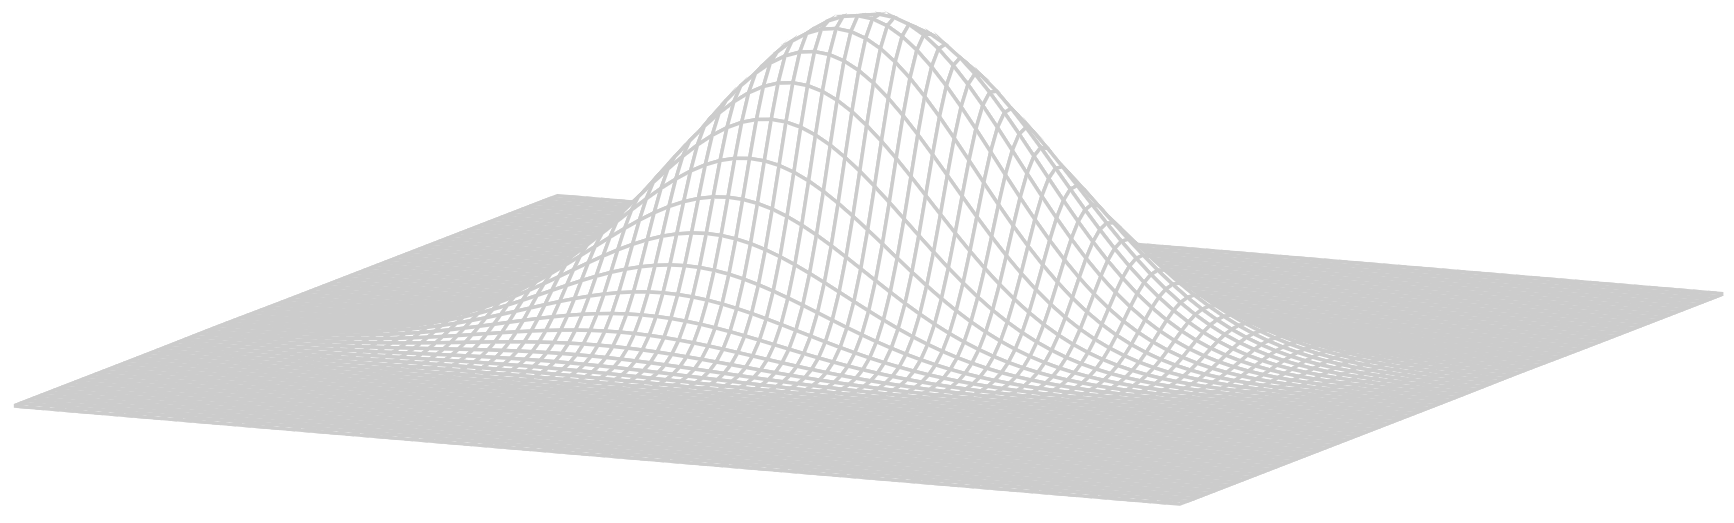
\includegraphics[scale=0.45]{bivar}
}\hfil}
Лінії рівня цієї поверхні задають \emph{еліпси розсіювання}:
$$f_{\vec{\xi}}(x,y) = C \Leftrightarrow \frac{(x-a_1)^2}{\sigma_1^2} -
2\rho\frac{x-a_1}{\sigma_1}\frac{y-a_2}{\sigma_2} +
\frac{(y-a_2)^2}{\sigma_2^2} = \lambda^2$$

\begin{tabular}{c p{7.8cm}}
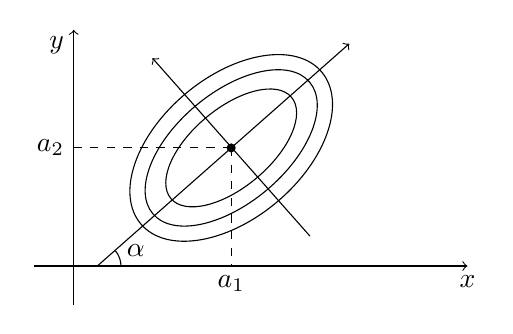
\begin{tikzpicture}[baseline={(current bounding box.north)}]
    \draw [->] (-0.5, 0) -- (5, 0);
    \draw [->] (0, -0.5) -- (0, 3);
    \draw (2, 1.5) circle [x radius=1, y radius=0.5, rotate=40];
    \draw (2, 1.5) circle [x radius=1.3, y radius=0.7, rotate=40];
    \draw (2, 1.5) circle [x radius=1.5, y radius=0.9, rotate=40];
    \draw [fill] (2, 1.5) circle [radius = 0.05];
    \draw [<-] (3.5, 2.824) -- (0.3, 0);
    \draw [<-] (1, 2.64) -- (3, 0.38);
    \draw [dashed] (2, 1.5) -- (0, 1.5);
    \draw [dashed] (2, 1.5) -- (2, 0);
    \node [below] at (5, 0) {$x$};
    \node [left] at (0, 2.8) {$y$};
    \node [below] at (2, 0) {$a_1$};
    \node [left] at (0, 1.5) {$a_2$};
    \draw (0.6, 0) arc (0:40:0.3);
    \node [above right] at (0.55, 0) {$\alpha$};
\end{tikzpicture}&
$\mathrm{tg}2\alpha = \frac{2\rho\sigma_1\sigma_2}{\sigma_1^2 - \sigma_2^2}$\newline
Осі еліпсів називаються \emph{головними осями розсіювання}.\newline
Якщо $\rho = 0$, то головні осі розсіювання паралельні осям координат.
\end{tabular}

Позначимо $E_\lambda = \left\{(x;y) \in \mathbb{R}^2: \frac{(x-a_1)^2}{\sigma_1^2} -
2\rho\frac{x-a_1}{\sigma_1}\frac{y-a_2}{\sigma_2} +
\frac{(y-a_2)^2}{\sigma_2^2} \leq \lambda^2\right\}$.
Знайдемо ймовірність потрапляння в цю область у випадку $\rho = 0$:

\begin{gather*}
    P\left\{\vec{\xi} \in E_\lambda\right\} = \iint\limits_{E_\lambda} f_{\vec{\xi}}(x,y) dx dy = 
    \frac{1}{2\pi\sigma_1\sigma_2} \iint\limits_{E_\lambda} \exp\left\{-\frac{1}{2}\left( 
        \frac{(x-a_1)^2}{\sigma_1^2} + 
        \frac{(y-a_2)^2}{\sigma_2^2}
    \right)\right\} dx dy = \\
    \left[ \begin{gathered}
        x-a_1 = \lambda\sigma_1 r \cos\varphi \\ 
        y-a_2 = \lambda\sigma_2 r \sin\varphi \\
        |\mathcal{J}| = \lambda^2 \sigma_1 \sigma_2 r
    \end{gathered}\right] = 
    \frac{\lambda^2}{2\pi} \int\limits_0^{2\pi}  d\varphi
    \int\limits_0^1 r e^{-\frac{\lambda^2r^2}{2}} dr = 
    \int\limits_0^1 e^{-\frac{\lambda^2r^2}{2}} d\left(\frac{\lambda^2r^2}{2} \right) = 
    1 - e^{-\frac{\lambda^2}{2}}
\end{gather*}

\begin{exercise}
    Довести, що у випадку $\rho > 0$ $P\left\{\vec{\xi} \in E_\lambda\right\} = 
    1 - e^{-\frac{\lambda^2}{2(1-\rho^2)}}$.
\end{exercise}

\begin{example}
    $\vec{\xi} \sim \mathrm{N}\left( \begin{pmatrix}
        -1 \\ 1
    \end{pmatrix}, \begin{pmatrix}
        1 & 2 \\
        2 & 16
    \end{pmatrix}\right)$. Знайти рівняння еліпса розсіювання, для якого \\
    $P\left\{\vec{\xi} \in E_\lambda\right\} = 0.93$. З кореляційної матриці $\rho = 0.5$.
    Розв'яжемо відносно $\lambda^2$ рівняння $1 - e^{-\frac{\lambda^2}{2(1-0.5^2)}} = 0.93
    \Leftrightarrow e^{-\frac{\lambda^2}{1.5}} = 0.07 \Rightarrow \lambda^2 \approx 4$. Тому рівняння еліпса
    $\frac{(x+1)^2}{1} - \frac{x+1}{1} \frac{y-1}{4} + \frac{(y-1)^2}{16} = 4$ або 
    $\frac{(x+1)^2}{4} - \frac{(x+1)(y-1)}{16} + \frac{(y-1)^2}{64} = 1$.
\end{example}

Розглянемо гауссівський вектор $\vec{\xi} = (\xi_1, \xi_2)$ з незалежними координатами.
Для нього $F_{\vec{\xi}}(x,y) = F_{\xi_1}(x) F_{\xi_2}(y) = 
\left(\frac{1}{2} + \Phi\left( \frac{x-a_1}{\sigma_1}\right) \right)
\left(\frac{1}{2} + \Phi\left( \frac{y-a_2}{\sigma_2}\right) \right)$.
Тоді ймовірність потрапляння в прямокутник $\Pi = \left\{(x;y)\in\mathbb{R}^2 : \alpha \leq x < \beta, \gamma \leq y < \delta\right\}$
дорівнює $$\left( \Phi\left( \frac{\beta-a_1}{\sigma_1}\right) - \Phi\left( \frac{\alpha-a_1}{\sigma_1}\right)\right) \cdot
\left( \Phi\left( \frac{\delta-a_2}{\sigma_2}\right) - \Phi\left( \frac{\gamma-a_2}{\sigma_2}\right)\right)$$
\begin{exercise}
    Довести формулу для $P\left\{\vec{\xi}\in\Pi\right\}$.
\end{exercise}
Для гауссівського вектору з незалежними координатами також має місце <<правило $3\sigma$>>:
\begin{gather*}
    P\left\{\vec{\xi} \in (a_1-3\sigma_1; a_1+3\sigma_1)\times(a_2-3\sigma_2; a_2+3\sigma_2)\right\} = \\
    = P\left\{\xi_1 \in(a_1-3\sigma_1; a_1+3\sigma_1)\right\}\cdot P\left\{\xi_2 \in(a_2-3\sigma_2; a_2+3\sigma_2)\right\}
    \approx 0.9973^2 \approx 0.9946
\end{gather*}

\subsection{Колове розсіювання}
\begin{definition}
    Двовимірний гауссівський вектор має \emph{колове розсіювання}, якщо
    $\vec{a} = \vec{0}, \; K = \begin{pmatrix}
        \sigma^2 & 0 \\
        0 & \sigma^2
    \end{pmatrix}$. В цьому випадку $f_{\vec{\xi}} = \frac{1}{2\pi\sigma^2} \exp\left\{-\frac{x^2+y^2}{2\sigma^2}\right\}$, 
    а еліпси розсіювання стають колами.
\end{definition}
Знайдемо ймовірність потрапляння такого $\vec{\xi}$ в коло $K_R = \left\{(x; y) \in \mathbb{R}^2 : x^2 + y^2 \leq R^2\right\}$:
\begin{gather*}
    P\left\{\vec{\xi} \in K_R\right\} = \frac{1}{2\pi\sigma^2} \iint\limits_{K_R} e^{-\frac{x^2+y^2}{2\sigma^2}} dx dy = 
    \left[ \begin{gathered}
        x = \sigma r\cos\varphi \\
        y = \sigma r\sin\varphi \\
        |\mathcal{J}| = \sigma^2 r
    \end{gathered}\right] =
    \frac{1}{2\pi} \int\limits_0^{2\pi} d\varphi \int\limits_0^{R/\sigma} r e^{-\frac{r^2}{2}} dr = \\
    = \int\limits_0^{R/\sigma} e^{-\frac{r^2}{2}} d \left( \frac{r^2}{2}\right) = 
    1 - e^{-\frac{R^2}{2\sigma^2}}
\end{gather*}
Таким чином, тепер відомий розподіл норми $\vec{\xi}$. $\eta = \Vert \vec{\xi} \Vert = \sqrt{\xi_1^2 + \xi_2^2}$ --- випадкова величина,
для якої $F_{\eta}(R) = P\left\{\Vert \vec{\xi} \Vert < R\right\} = \begin{cases}
    1 - e^{-\frac{R^2}{2\sigma^2}}, & R > 0 \\
    0, & R \leq 0
\end{cases}$ --- це \emph{розподіл Релея}. Ця властивість переноситься й на довільну скінченну розмірність.

\begin{exercise}
    Знайти основні числові характеристики розподілу Релея.
\end{exercise}

\subsection{Умовний гауссівський розподіл на площині}
Знайдемо одну з умовних щільностей розподілу:
\begin{gather*}
    f_{\xi_1}(x/\xi_2 = y) = \frac{f_{\vec{\xi}}(x,y)}{f_{\xi_2}(y)} = 
    \frac{\frac{1}{2\pi\sigma_1\sigma_2\sqrt{1-\rho^2}} \exp\left\{
        -\frac{1}{2(1-\rho^2)}\cdot
        \left(\frac{(x-a_1)^2}{\sigma_1^2} -
        2\rho\frac{x-a_1}{\sigma_1}\frac{y-a_2}{\sigma_2} +
        \frac{(y-a_2)^2}{\sigma_2^2}
        \right)\right\} }{
            \frac{1}{\sqrt{2\pi}\sigma_2} \exp\left\{-\frac{1}{2\sigma_2^2}(y-a_2)^2\right\}
        } = \\
        \frac{1}{\sqrt{2\pi}\sigma_1\sqrt{1-\rho^2}} \exp\left\{
            -\frac{1}{2(1-\rho^2)}
        \left(\frac{(x-a_1)^2}{\sigma_1^2} -
        2\rho\frac{(x-a_1)(y-a_2)}{\sigma_1\sigma_2} +
        \frac{(y-a_2)^2}{\sigma_2^2}
        \right) +
        \frac{(y-a_2)^2}{2\sigma_2^2}
        \right\} = \\
        = \left [ \frac{(y-a_2)^2}{\sigma_2^2} - \frac{(1-\rho^2)(y-a_2)^2}{\sigma_2^2} = \rho^2 \frac{(y-a_2)^2}{\sigma_2^2}\right]=\\
        = \frac{1}{\sqrt{2\pi}\sigma_1\sqrt{1-\rho^2}} \exp\left\{-\frac{1}{2(1-\rho^2)}\left( \frac{x-a_1}{\sigma_1} - \rho\cdot\frac{y-a_2}{\sigma_2}\right)^2\right\} = \\
        = \frac{1}{\sqrt{2\pi}\sigma_1\sqrt{1-\rho^2}} \exp\left\{-\frac{1}{2\sigma_1^2(1-\rho^2)}\left( x- \left( a_1 + \frac{\rho\sigma_1(y-a_2)}{\sigma_2}\right)\right)^2\right\}
\end{gather*}
Аналогічно $f_{\xi_2}(y/\xi_1 = x) = \frac{1}{\sqrt{2\pi}\sigma_2\sqrt{1-\rho^2}} \exp\left\{-\frac{1}{2\sigma_2^2(1-\rho^2)}\left( y- \left( a_2 + \frac{\rho\sigma_2(x-a_1)}{\sigma_1}\right)\right)^2\right\}$.

\noindentОтже, обидві умовні щільності є щільностями нормального розподілу.

$E\left( \xi_1 / \xi_2 = y\right) = a_1 + \frac{\rho\sigma_1(y-a_2)}{\sigma_2}$, 
$E\left( \xi_2 / \xi_1 = x\right) = a_2 + \frac{\rho\sigma_2(x-a_1)}{\sigma_1}$. Лінії регресії --- прямі,

\noindent
$\rho\frac{\sigma_1}{\sigma_2} = \frac{K\xi_1\xi_2}{D\xi_2}$ та $\rho\frac{\sigma_2}{\sigma_1}  = \frac{K\xi_1\xi_2}{D\xi_1}$ --- відповідні кутові коефіцієнти прямих регресії.

$D\left( \xi_1 / \xi_2 = y\right) = \sigma_1^2(1-\rho^2)$, 
$D\left( \xi_2 / \xi_1 = x\right) = \sigma_2^2(1-\rho^2)$. Умовні дисперсії є сталими, ця властивість називається \emph{гомоскедастичністю}.